\documentclass[twoside]{book}

% Packages required by doxygen
\usepackage{fixltx2e}
\usepackage{calc}
\usepackage{doxygen}
\usepackage[export]{adjustbox} % also loads graphicx
\usepackage{graphicx}
\usepackage[utf8]{inputenc}
\usepackage{makeidx}
\usepackage{multicol}
\usepackage{multirow}
\PassOptionsToPackage{warn}{textcomp}
\usepackage{textcomp}
\usepackage[nointegrals]{wasysym}
\usepackage[table]{xcolor}

% Font selection
\usepackage[T1]{fontenc}
\usepackage[scaled=.90]{helvet}
\usepackage{courier}
\usepackage{amssymb}
\usepackage{sectsty}
\renewcommand{\familydefault}{\sfdefault}
\allsectionsfont{%
  \fontseries{bc}\selectfont%
  \color{darkgray}%
}
\renewcommand{\DoxyLabelFont}{%
  \fontseries{bc}\selectfont%
  \color{darkgray}%
}
\newcommand{\+}{\discretionary{\mbox{\scriptsize$\hookleftarrow$}}{}{}}

% Page & text layout
\usepackage{geometry}
\geometry{%
  a4paper,%
  top=2.5cm,%
  bottom=2.5cm,%
  left=2.5cm,%
  right=2.5cm%
}
\tolerance=750
\hfuzz=15pt
\hbadness=750
\setlength{\emergencystretch}{15pt}
\setlength{\parindent}{0cm}
\setlength{\parskip}{0.2cm}
\makeatletter
\renewcommand{\paragraph}{%
  \@startsection{paragraph}{4}{0ex}{-1.0ex}{1.0ex}{%
    \normalfont\normalsize\bfseries\SS@parafont%
  }%
}
\renewcommand{\subparagraph}{%
  \@startsection{subparagraph}{5}{0ex}{-1.0ex}{1.0ex}{%
    \normalfont\normalsize\bfseries\SS@subparafont%
  }%
}
\makeatother

% Headers & footers
\usepackage{fancyhdr}
\pagestyle{fancyplain}
\fancyhead[LE]{\fancyplain{}{\bfseries\thepage}}
\fancyhead[CE]{\fancyplain{}{}}
\fancyhead[RE]{\fancyplain{}{\bfseries\leftmark}}
\fancyhead[LO]{\fancyplain{}{\bfseries\rightmark}}
\fancyhead[CO]{\fancyplain{}{}}
\fancyhead[RO]{\fancyplain{}{\bfseries\thepage}}
\fancyfoot[LE]{\fancyplain{}{}}
\fancyfoot[CE]{\fancyplain{}{}}
\fancyfoot[RE]{\fancyplain{}{\bfseries\scriptsize Generated on Wed Apr 29 2015 20\+:28\+:20 for Cast into the Voidstar by Doxygen }}
\fancyfoot[LO]{\fancyplain{}{\bfseries\scriptsize Generated on Wed Apr 29 2015 20\+:28\+:20 for Cast into the Voidstar by Doxygen }}
\fancyfoot[CO]{\fancyplain{}{}}
\fancyfoot[RO]{\fancyplain{}{}}
\renewcommand{\footrulewidth}{0.4pt}
\renewcommand{\chaptermark}[1]{%
  \markboth{#1}{}%
}
\renewcommand{\sectionmark}[1]{%
  \markright{\thesection\ #1}%
}

% Indices & bibliography
\usepackage{natbib}
\usepackage[titles]{tocloft}
\setcounter{tocdepth}{3}
\setcounter{secnumdepth}{5}
\makeindex

% Hyperlinks (required, but should be loaded last)
\usepackage{ifpdf}
\ifpdf
  \usepackage[pdftex,pagebackref=true]{hyperref}
\else
  \usepackage[ps2pdf,pagebackref=true]{hyperref}
\fi
\hypersetup{%
  colorlinks=true,%
  linkcolor=blue,%
  citecolor=blue,%
  unicode%
}

% Custom commands
\newcommand{\clearemptydoublepage}{%
  \newpage{\pagestyle{empty}\cleardoublepage}%
}


%===== C O N T E N T S =====

\begin{document}

% Titlepage & ToC
\hypersetup{pageanchor=false,
             bookmarks=true,
             bookmarksnumbered=true,
             pdfencoding=unicode
            }
\pagenumbering{roman}
\begin{titlepage}
\vspace*{7cm}
\begin{center}%
{\Large Cast into the Voidstar \\[1ex]\large 0.\+02 }\\
\vspace*{1cm}
{\large Generated by Doxygen 1.8.9.1}\\
\vspace*{0.5cm}
{\small Wed Apr 29 2015 20:28:20}\\
\end{center}
\end{titlepage}
\clearemptydoublepage
\tableofcontents
\clearemptydoublepage
\pagenumbering{arabic}
\hypersetup{pageanchor=true}

%--- Begin generated contents ---
\chapter{Hierarchical Index}
\section{Class Hierarchy}
This inheritance list is sorted roughly, but not completely, alphabetically\+:\begin{DoxyCompactList}
\item \contentsline{section}{Enemy\+Controller.\+Agent}{\pageref{class_enemy_controller_1_1_agent}}{}
\item \contentsline{section}{A\+I\+Controller.\+A\+I\+State}{\pageref{class_a_i_controller_1_1_a_i_state}}{}
\item \contentsline{section}{Asteroid\+Controller.\+Building}{\pageref{class_asteroid_controller_1_1_building}}{}
\item Mono\+Behaviour\begin{DoxyCompactList}
\item \contentsline{section}{A\+I\+Controller}{\pageref{class_a_i_controller}}{}
\item \contentsline{section}{Asteroid\+Controller}{\pageref{class_asteroid_controller}}{}
\item \contentsline{section}{Enemy\+Controller}{\pageref{class_enemy_controller}}{}
\item \contentsline{section}{Game\+Controller}{\pageref{class_game_controller}}{}
\item \contentsline{section}{Shot}{\pageref{class_shot}}{}
\item \contentsline{section}{Unit\+Controller}{\pageref{class_unit_controller}}{}
\end{DoxyCompactList}
\item \contentsline{section}{Game\+Controller.\+Player}{\pageref{class_game_controller_1_1_player}}{}
\end{DoxyCompactList}

\chapter{Class Index}
\section{Class List}
Here are the classes, structs, unions and interfaces with brief descriptions\+:\begin{DoxyCompactList}
\item\contentsline{section}{\hyperlink{class_enemy_controller_1_1_agent}{Enemy\+Controller.\+Agent} }{\pageref{class_enemy_controller_1_1_agent}}{}
\item\contentsline{section}{\hyperlink{class_a_i_controller}{A\+I\+Controller} }{\pageref{class_a_i_controller}}{}
\item\contentsline{section}{\hyperlink{class_a_i_controller_1_1_a_i_state}{A\+I\+Controller.\+A\+I\+State} }{\pageref{class_a_i_controller_1_1_a_i_state}}{}
\item\contentsline{section}{\hyperlink{class_android}{Android} }{\pageref{class_android}}{}
\item\contentsline{section}{\hyperlink{class_asteroid_controller}{Asteroid\+Controller} }{\pageref{class_asteroid_controller}}{}
\item\contentsline{section}{\hyperlink{class_asteroid_controller_1_1_building}{Asteroid\+Controller.\+Building} }{\pageref{class_asteroid_controller_1_1_building}}{}
\item\contentsline{section}{\hyperlink{class_enemy_controller}{Enemy\+Controller} }{\pageref{class_enemy_controller}}{}
\item\contentsline{section}{\hyperlink{class_game_controller}{Game\+Controller} }{\pageref{class_game_controller}}{}
\item\contentsline{section}{\hyperlink{class_g_u_i}{G\+U\+I} }{\pageref{class_g_u_i}}{}
\item\contentsline{section}{\hyperlink{class_menu}{Menu} }{\pageref{class_menu}}{}
\item\contentsline{section}{\hyperlink{class_mothership_controller}{Mothership\+Controller} }{\pageref{class_mothership_controller}}{}
\item\contentsline{section}{\hyperlink{class_game_controller_1_1_player}{Game\+Controller.\+Player} }{\pageref{class_game_controller_1_1_player}}{}
\item\contentsline{section}{\hyperlink{class_shot}{Shot} }{\pageref{class_shot}}{}
\item\contentsline{section}{\hyperlink{class_touch_script}{Touch\+Script} }{\pageref{class_touch_script}}{}
\item\contentsline{section}{\hyperlink{class_unit_controller}{Unit\+Controller} }{\pageref{class_unit_controller}}{}
\end{DoxyCompactList}

\chapter{Class Documentation}
\hypertarget{class_enemy_controller_1_1_agent}{}\section{Enemy\+Controller.\+Agent Class Reference}
\label{class_enemy_controller_1_1_agent}\index{Enemy\+Controller.\+Agent@{Enemy\+Controller.\+Agent}}
\subsection*{Public Member Functions}
\begin{DoxyCompactItemize}
\item 
\hypertarget{class_enemy_controller_1_1_agent_a2be9541303a366a0c46a38df9a8c0200}{}{\bfseries Agent} (float agg, float def)\label{class_enemy_controller_1_1_agent_a2be9541303a366a0c46a38df9a8c0200}

\item 
\hypertarget{class_enemy_controller_1_1_agent_a9a42f29b3793b887b5b9fbb9b7764976}{}void {\bfseries set\+Asteroid} (Game\+Object astero)\label{class_enemy_controller_1_1_agent_a9a42f29b3793b887b5b9fbb9b7764976}

\item 
\hypertarget{class_enemy_controller_1_1_agent_a28475b138ec51dc83ad1abbf6b8d7cc0}{}Game\+Object {\bfseries get\+Asteroid} ()\label{class_enemy_controller_1_1_agent_a28475b138ec51dc83ad1abbf6b8d7cc0}

\item 
\hypertarget{class_enemy_controller_1_1_agent_a0a89319a0e8f1ab5a16781feb601f4f5}{}void {\bfseries set\+Time\+Passed} (float f)\label{class_enemy_controller_1_1_agent_a0a89319a0e8f1ab5a16781feb601f4f5}

\item 
\hypertarget{class_enemy_controller_1_1_agent_a78f5488f282910c7b71db69a94cc3836}{}float {\bfseries get\+Time\+Passed} ()\label{class_enemy_controller_1_1_agent_a78f5488f282910c7b71db69a94cc3836}

\item 
\hypertarget{class_enemy_controller_1_1_agent_a0b09c672b766b14187aacf80caf5af17}{}void {\bfseries set\+Capping} (float f)\label{class_enemy_controller_1_1_agent_a0b09c672b766b14187aacf80caf5af17}

\item 
\hypertarget{class_enemy_controller_1_1_agent_a6359b5e60bd6e61e068a688f419af3d8}{}float {\bfseries get\+Capping} ()\label{class_enemy_controller_1_1_agent_a6359b5e60bd6e61e068a688f419af3d8}

\item 
\hypertarget{class_enemy_controller_1_1_agent_aeb949646839bdeaa177d4a7596c3b07a}{}void {\bfseries set\+Destination} (Vector3 pos)\label{class_enemy_controller_1_1_agent_aeb949646839bdeaa177d4a7596c3b07a}

\item 
\hypertarget{class_enemy_controller_1_1_agent_aef6481f39c1b4bc673f33b61691bb90d}{}Vector3 {\bfseries get\+Destination} ()\label{class_enemy_controller_1_1_agent_aef6481f39c1b4bc673f33b61691bb90d}

\item 
\hypertarget{class_enemy_controller_1_1_agent_a651ff5b9d8a6664100d76726e0f9765e}{}void {\bfseries set\+Aggresivness} (float f)\label{class_enemy_controller_1_1_agent_a651ff5b9d8a6664100d76726e0f9765e}

\item 
\hypertarget{class_enemy_controller_1_1_agent_a0be4af1e7ded9baaa77a6716db289a03}{}void {\bfseries set\+Defensivness} (float f)\label{class_enemy_controller_1_1_agent_a0be4af1e7ded9baaa77a6716db289a03}

\item 
\hypertarget{class_enemy_controller_1_1_agent_a865449479179cccb49cb3e0724842742}{}void {\bfseries set\+Strength} (float f)\label{class_enemy_controller_1_1_agent_a865449479179cccb49cb3e0724842742}

\item 
\hypertarget{class_enemy_controller_1_1_agent_abccb50c8d632abd1613fd7bb590aca2d}{}void {\bfseries set\+Group\+Strength} (float f)\label{class_enemy_controller_1_1_agent_abccb50c8d632abd1613fd7bb590aca2d}

\item 
\hypertarget{class_enemy_controller_1_1_agent_a79705a445e3452bc96fd3150a4521ab8}{}void {\bfseries set\+Target} (Game\+Object go)\label{class_enemy_controller_1_1_agent_a79705a445e3452bc96fd3150a4521ab8}

\item 
\hypertarget{class_enemy_controller_1_1_agent_aa520331274e0a39f6587f3dddbcef7df}{}Game\+Object {\bfseries get\+Target} ()\label{class_enemy_controller_1_1_agent_aa520331274e0a39f6587f3dddbcef7df}

\item 
\hypertarget{class_enemy_controller_1_1_agent_aa49ed546f0ed6a06f554a386607582df}{}void {\bfseries set\+Transform} (Transform t)\label{class_enemy_controller_1_1_agent_aa49ed546f0ed6a06f554a386607582df}

\item 
\hypertarget{class_enemy_controller_1_1_agent_afa53d87289c4af17cb407e391a03da14}{}Transform {\bfseries get\+Transform} ()\label{class_enemy_controller_1_1_agent_afa53d87289c4af17cb407e391a03da14}

\item 
\hypertarget{class_enemy_controller_1_1_agent_ad2e67bdc0957aa906a427e7b385a1bb6}{}void {\bfseries add\+Enemy} (Game\+Object enemy)\label{class_enemy_controller_1_1_agent_ad2e67bdc0957aa906a427e7b385a1bb6}

\item 
\hypertarget{class_enemy_controller_1_1_agent_af2e214b9a964b8277c4f97ff9c762251}{}void {\bfseries remove\+Enemy} (Game\+Object enemy)\label{class_enemy_controller_1_1_agent_af2e214b9a964b8277c4f97ff9c762251}

\item 
\hypertarget{class_enemy_controller_1_1_agent_a16c99220f5df752bd3bbedaa0188418e}{}void {\bfseries add\+Ally} (Game\+Object ally)\label{class_enemy_controller_1_1_agent_a16c99220f5df752bd3bbedaa0188418e}

\item 
\hypertarget{class_enemy_controller_1_1_agent_acd0813f8ea5ba116c5cb700e4dc1004f}{}void {\bfseries remove\+Ally} (Game\+Object ally)\label{class_enemy_controller_1_1_agent_acd0813f8ea5ba116c5cb700e4dc1004f}

\item 
\hypertarget{class_enemy_controller_1_1_agent_ad41969970fdcfc56ddd475c0ceea04bb}{}void {\bfseries flee} ()\label{class_enemy_controller_1_1_agent_ad41969970fdcfc56ddd475c0ceea04bb}

\item 
\hypertarget{class_enemy_controller_1_1_agent_a5c50a2432bf00a04e1365758d7182ee1}{}void {\bfseries scout} ()\label{class_enemy_controller_1_1_agent_a5c50a2432bf00a04e1365758d7182ee1}

\item 
\hypertarget{class_enemy_controller_1_1_agent_ad54d26eeeac1c75cf491c50765da9c97}{}bool {\bfseries call\+For\+Backup} ()\label{class_enemy_controller_1_1_agent_ad54d26eeeac1c75cf491c50765da9c97}

\item 
\hypertarget{class_enemy_controller_1_1_agent_a1d0126f3f76ef35fd0fe91a2e976af8f}{}void {\bfseries think} ()\label{class_enemy_controller_1_1_agent_a1d0126f3f76ef35fd0fe91a2e976af8f}

\end{DoxyCompactItemize}


The documentation for this class was generated from the following file\+:\begin{DoxyCompactItemize}
\item 
Assets/\+Scripts/Enemy\+Controller.\+cs\end{DoxyCompactItemize}

\hypertarget{class_a_i_controller}{}\section{A\+I\+Controller Class Reference}
\label{class_a_i_controller}\index{A\+I\+Controller@{A\+I\+Controller}}
Inheritance diagram for A\+I\+Controller\+:\begin{figure}[H]
\begin{center}
\leavevmode
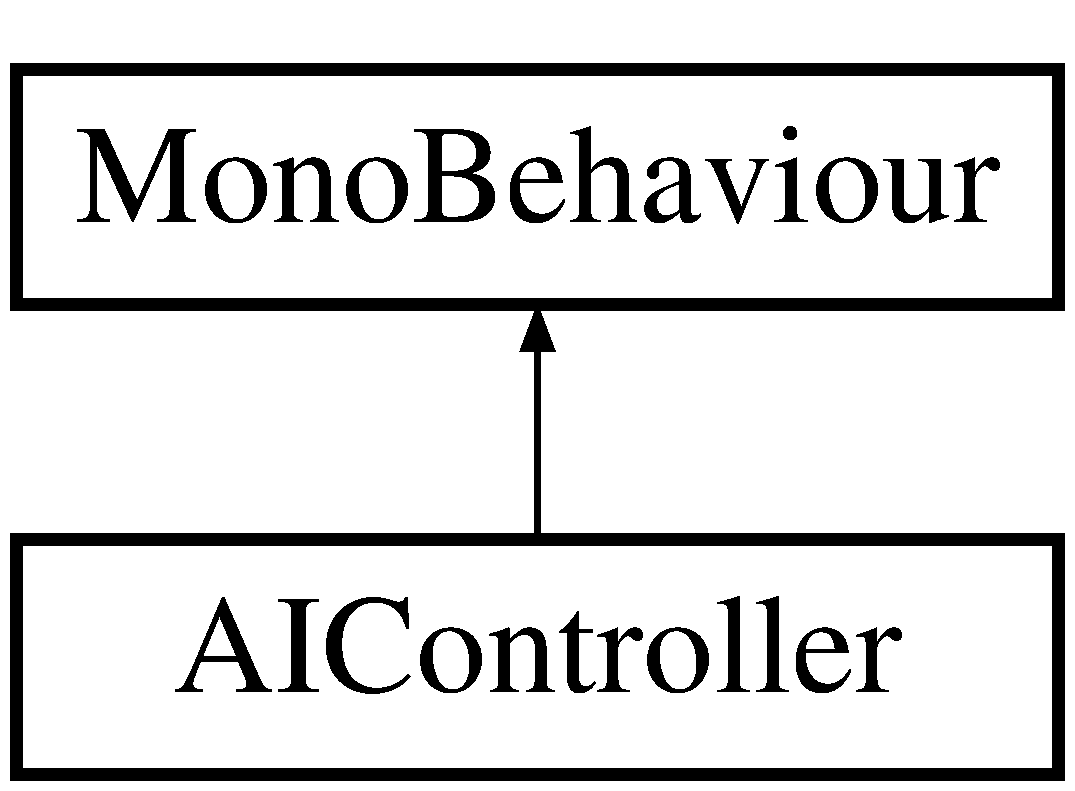
\includegraphics[height=2.000000cm]{class_a_i_controller}
\end{center}
\end{figure}
\subsection*{Classes}
\begin{DoxyCompactItemize}
\item 
class \hyperlink{class_a_i_controller_1_1_a_i_state}{A\+I\+State}
\end{DoxyCompactItemize}
\subsection*{Public Member Functions}
\begin{DoxyCompactItemize}
\item 
\hypertarget{class_a_i_controller_a2def6727dc18d551ed80734d40853ae0}{}bool {\bfseries requested\+Backup} (Game\+Object go)\label{class_a_i_controller_a2def6727dc18d551ed80734d40853ae0}

\item 
\hypertarget{class_a_i_controller_a8124de03eacb145d9187a1c6139417da}{}void {\bfseries record\+Knowledge} ()\label{class_a_i_controller_a8124de03eacb145d9187a1c6139417da}

\item 
\hypertarget{class_a_i_controller_ab91b933e115fe715a2a32ea00336c05f}{}void {\bfseries reported\+Enemy} (Game\+Object go)\label{class_a_i_controller_ab91b933e115fe715a2a32ea00336c05f}

\item 
\hypertarget{class_a_i_controller_a90cd1325dbe011127063e5e099372165}{}void {\bfseries change\+Units\+Behaviour} ()\label{class_a_i_controller_a90cd1325dbe011127063e5e099372165}

\item 
\hypertarget{class_a_i_controller_a637c90cb0057aab98431c62b8257e9f4}{}void {\bfseries load\+Params} (\hyperlink{class_a_i_controller_1_1_a_i_state}{A\+I\+State} state)\label{class_a_i_controller_a637c90cb0057aab98431c62b8257e9f4}

\item 
\hypertarget{class_a_i_controller_ac868ca1d10ccf1455a13f88b5f849401}{}void {\bfseries rethink\+My\+Actions} ()\label{class_a_i_controller_ac868ca1d10ccf1455a13f88b5f849401}

\item 
\hypertarget{class_a_i_controller_a051753509a5e22829dadf3bb08eccd48}{}void {\bfseries update\+Values} ()\label{class_a_i_controller_a051753509a5e22829dadf3bb08eccd48}

\item 
\hypertarget{class_a_i_controller_a348e9c5bd9e3ef59523577058524b034}{}void {\bfseries delete\+Unit} (Game\+Object unit)\label{class_a_i_controller_a348e9c5bd9e3ef59523577058524b034}

\item 
\hypertarget{class_a_i_controller_aa7f409a237a65ef7757e60947e3ad8b9}{}void {\bfseries build\+Unit} ()\label{class_a_i_controller_aa7f409a237a65ef7757e60947e3ad8b9}

\end{DoxyCompactItemize}
\subsection*{Public Attributes}
\begin{DoxyCompactItemize}
\item 
\hypertarget{class_a_i_controller_a4b8a5c97c0fb6cf61eec392547a3514f}{}Hash\+Set$<$ Game\+Object $>$ {\bfseries units}\label{class_a_i_controller_a4b8a5c97c0fb6cf61eec392547a3514f}

\item 
\hypertarget{class_a_i_controller_a94a988b0c68154f5437c3254e229ec8c}{}Hash\+Set$<$ Game\+Object $>$ {\bfseries enemies}\label{class_a_i_controller_a94a988b0c68154f5437c3254e229ec8c}

\item 
\hypertarget{class_a_i_controller_ae6e9e675c8cfa60e56721cb0da4010bf}{}Game\+Object {\bfseries mothership}\label{class_a_i_controller_ae6e9e675c8cfa60e56721cb0da4010bf}

\end{DoxyCompactItemize}


The documentation for this class was generated from the following file\+:\begin{DoxyCompactItemize}
\item 
Assets/\+Scripts/A\+I\+Controller.\+cs\end{DoxyCompactItemize}

\hypertarget{class_a_i_controller_1_1_a_i_state}{}\section{A\+I\+Controller.\+A\+I\+State Class Reference}
\label{class_a_i_controller_1_1_a_i_state}\index{A\+I\+Controller.\+A\+I\+State@{A\+I\+Controller.\+A\+I\+State}}
\subsection*{Public Member Functions}
\begin{DoxyCompactItemize}
\item 
\hypertarget{class_a_i_controller_1_1_a_i_state_af8a3df1714218ae8ec1a6e7d2db440a1}{}{\bfseries A\+I\+State} (float a, float d, int nu, int eu, float p, float ep, float na, float c)\label{class_a_i_controller_1_1_a_i_state_af8a3df1714218ae8ec1a6e7d2db440a1}

\item 
\hypertarget{class_a_i_controller_1_1_a_i_state_a674181d9ff21c9ae3cae181b21150ea3}{}float {\bfseries calculate\+State} ()\label{class_a_i_controller_1_1_a_i_state_a674181d9ff21c9ae3cae181b21150ea3}

\end{DoxyCompactItemize}
\subsection*{Public Attributes}
\begin{DoxyCompactItemize}
\item 
\hypertarget{class_a_i_controller_1_1_a_i_state_ac322a22e73dd6159e83649fdb754e738}{}float {\bfseries aggresivness}\label{class_a_i_controller_1_1_a_i_state_ac322a22e73dd6159e83649fdb754e738}

\item 
\hypertarget{class_a_i_controller_1_1_a_i_state_a37bf9e7234c9d32f606b073cc20cf96a}{}float {\bfseries defensivness}\label{class_a_i_controller_1_1_a_i_state_a37bf9e7234c9d32f606b073cc20cf96a}

\item 
\hypertarget{class_a_i_controller_1_1_a_i_state_a8711f514c2794b832cced06277497d42}{}int {\bfseries num\+Of\+Units}\label{class_a_i_controller_1_1_a_i_state_a8711f514c2794b832cced06277497d42}

\item 
\hypertarget{class_a_i_controller_1_1_a_i_state_a7eec1e67aa6c7ddc07bf395bc87e0f88}{}int {\bfseries enemy\+Units}\label{class_a_i_controller_1_1_a_i_state_a7eec1e67aa6c7ddc07bf395bc87e0f88}

\item 
\hypertarget{class_a_i_controller_1_1_a_i_state_a6c47557910a46907b216f583aea42495}{}float {\bfseries points}\label{class_a_i_controller_1_1_a_i_state_a6c47557910a46907b216f583aea42495}

\item 
\hypertarget{class_a_i_controller_1_1_a_i_state_a800d73bdf57da35525bf0c48ba16566b}{}float {\bfseries enemy\+Points}\label{class_a_i_controller_1_1_a_i_state_a800d73bdf57da35525bf0c48ba16566b}

\item 
\hypertarget{class_a_i_controller_1_1_a_i_state_a156330391c48aead4c966159e13171b7}{}float {\bfseries num\+Of\+Asteroids}\label{class_a_i_controller_1_1_a_i_state_a156330391c48aead4c966159e13171b7}

\item 
\hypertarget{class_a_i_controller_1_1_a_i_state_a27c6681fb9475fe31d5b4f505b30e961}{}float {\bfseries credits}\label{class_a_i_controller_1_1_a_i_state_a27c6681fb9475fe31d5b4f505b30e961}

\end{DoxyCompactItemize}


The documentation for this class was generated from the following file\+:\begin{DoxyCompactItemize}
\item 
C\+:/\+Users/\+Franek/\+Documents/\+Cast into the Voidstar/\+Assets/\+Scripts/A\+I\+Controller.\+cs\end{DoxyCompactItemize}

\hypertarget{class_asteroid_controller}{}\section{Asteroid\+Controller Class Reference}
\label{class_asteroid_controller}\index{Asteroid\+Controller@{Asteroid\+Controller}}
Inheritance diagram for Asteroid\+Controller\+:\begin{figure}[H]
\begin{center}
\leavevmode
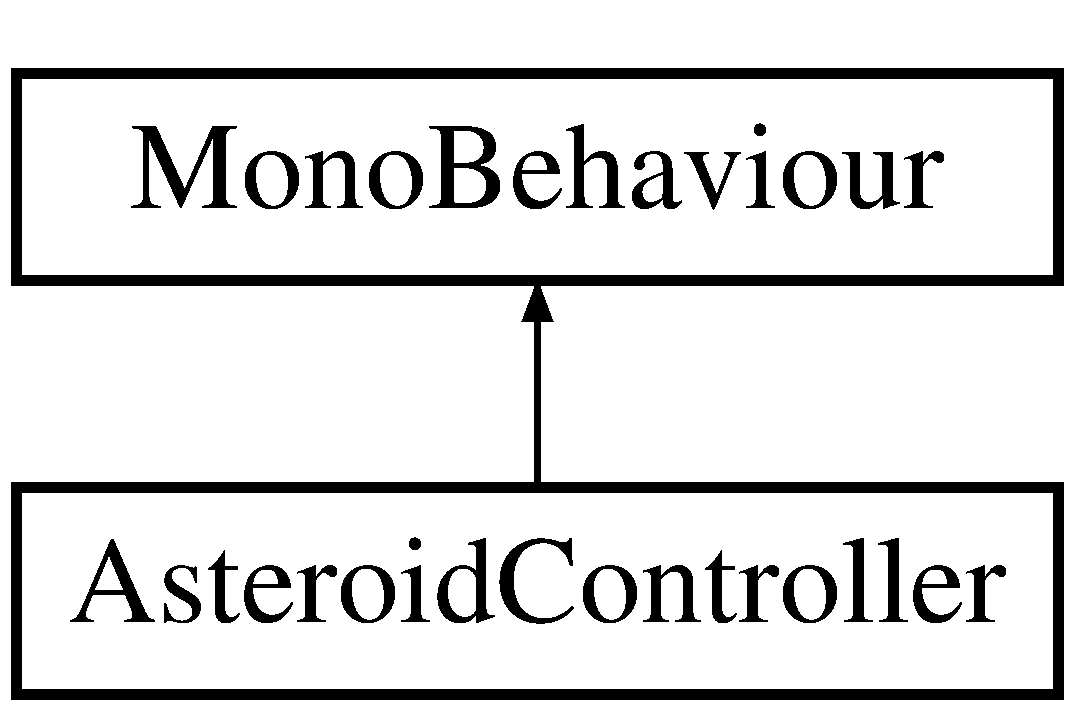
\includegraphics[height=2.000000cm]{class_asteroid_controller}
\end{center}
\end{figure}
\subsection*{Classes}
\begin{DoxyCompactItemize}
\item 
class \hyperlink{class_asteroid_controller_1_1_building}{Building}
\end{DoxyCompactItemize}
\subsection*{Public Types}
\begin{DoxyCompactItemize}
\item 
\hypertarget{class_asteroid_controller_a6203d45c2ca3e0538b31a8335a936266}{}enum {\bfseries Master} \{ {\bfseries Player}, 
{\bfseries Enemy}, 
{\bfseries None}
 \}\label{class_asteroid_controller_a6203d45c2ca3e0538b31a8335a936266}

\end{DoxyCompactItemize}
\subsection*{Public Member Functions}
\begin{DoxyCompactItemize}
\item 
\hypertarget{class_asteroid_controller_adbba795cc94547b904b76ee5538dd59f}{}bool {\bfseries create\+Building} (Master player)\label{class_asteroid_controller_adbba795cc94547b904b76ee5538dd59f}

\item 
\hypertarget{class_asteroid_controller_ab363019e3e8cea23f88d00f0414dcbf7}{}bool {\bfseries attack\+Building} (Game\+Object unit)\label{class_asteroid_controller_ab363019e3e8cea23f88d00f0414dcbf7}

\item 
\hypertarget{class_asteroid_controller_afe37fe0c1d100561f22df54af83aa730}{}bool {\bfseries attack\+Building} (List$<$ Game\+Object $>$ units)\label{class_asteroid_controller_afe37fe0c1d100561f22df54af83aa730}

\item 
\hypertarget{class_asteroid_controller_ac398b7ee353b74a40fba38a9438ba2bb}{}bool {\bfseries destroy\+Building} ()\label{class_asteroid_controller_ac398b7ee353b74a40fba38a9438ba2bb}

\item 
\hypertarget{class_asteroid_controller_a1cda3a360b1b402d2cfb020379e70ccf}{}void {\bfseries unit\+Killed} (Game\+Object unit)\label{class_asteroid_controller_a1cda3a360b1b402d2cfb020379e70ccf}

\item 
\hypertarget{class_asteroid_controller_a3d51e1ac2d51dc0c8e55186d0042336f}{}\hyperlink{class_asteroid_controller_1_1_building}{Building} {\bfseries get\+Building} ()\label{class_asteroid_controller_a3d51e1ac2d51dc0c8e55186d0042336f}

\end{DoxyCompactItemize}
\subsection*{Static Public Member Functions}
\begin{DoxyCompactItemize}
\item 
\hypertarget{class_asteroid_controller_acc4302a7a420e00f85397ab0f89b5215}{}static Master {\bfseries get\+Player} (Game\+Object ob)\label{class_asteroid_controller_acc4302a7a420e00f85397ab0f89b5215}

\end{DoxyCompactItemize}
\subsection*{Public Attributes}
\begin{DoxyCompactItemize}
\item 
\hypertarget{class_asteroid_controller_a1a82623f0a5fbab9d9abf8608c2db739}{}float {\bfseries capture\+Range\+Sqr} = 4900.\+0f\label{class_asteroid_controller_a1a82623f0a5fbab9d9abf8608c2db739}

\item 
\hypertarget{class_asteroid_controller_a450dcd7944d45dc1055950b6ba42dae8}{}Game\+Object {\bfseries prefab\+Building\+Model}\label{class_asteroid_controller_a450dcd7944d45dc1055950b6ba42dae8}

\item 
\hypertarget{class_asteroid_controller_a3d499ebc9c4556776a3b736664f2a1a5}{}Game\+Object {\bfseries prefab\+Enemy\+Building\+Model}\label{class_asteroid_controller_a3d499ebc9c4556776a3b736664f2a1a5}

\item 
\hypertarget{class_asteroid_controller_a5980b7670033334fe07315a63540d192}{}Master {\bfseries belongs\+To}\label{class_asteroid_controller_a5980b7670033334fe07315a63540d192}

\end{DoxyCompactItemize}


The documentation for this class was generated from the following file\+:\begin{DoxyCompactItemize}
\item 
Assets/\+Scripts/Asteroid\+Controller.\+cs\end{DoxyCompactItemize}

\hypertarget{class_asteroid_controller_1_1_building}{}\section{Asteroid\+Controller.\+Building Class Reference}
\label{class_asteroid_controller_1_1_building}\index{Asteroid\+Controller.\+Building@{Asteroid\+Controller.\+Building}}
\subsection*{Public Member Functions}
\begin{DoxyCompactItemize}
\item 
\hypertarget{class_asteroid_controller_1_1_building_ac4c0a79f7a3c8283448d0ec492567088}{}{\bfseries Building} (Master who, Game\+Object b)\label{class_asteroid_controller_1_1_building_ac4c0a79f7a3c8283448d0ec492567088}

\item 
\hypertarget{class_asteroid_controller_1_1_building_a251816c3dbfdc0628616dd0b16a52953}{}void {\bfseries update\+On\+Creation} (float t)\label{class_asteroid_controller_1_1_building_a251816c3dbfdc0628616dd0b16a52953}

\item 
\hypertarget{class_asteroid_controller_1_1_building_aa459e03784cd13bb7721a45a410f6676}{}void {\bfseries destroy\+Building} ()\label{class_asteroid_controller_1_1_building_aa459e03784cd13bb7721a45a410f6676}

\item 
\hypertarget{class_asteroid_controller_1_1_building_a924015ad91f9057bc12339a629e7f478}{}Game\+Object {\bfseries get\+Building} ()\label{class_asteroid_controller_1_1_building_a924015ad91f9057bc12339a629e7f478}

\item 
\hypertarget{class_asteroid_controller_1_1_building_ad9f7cc6118bc26552a28bed625a0b4e4}{}Master {\bfseries who\+Controlls} ()\label{class_asteroid_controller_1_1_building_ad9f7cc6118bc26552a28bed625a0b4e4}

\item 
\hypertarget{class_asteroid_controller_1_1_building_a08c8ffcba512689bda4c6ac59f2e8a18}{}float {\bfseries get\+H\+P} ()\label{class_asteroid_controller_1_1_building_a08c8ffcba512689bda4c6ac59f2e8a18}

\item 
\hypertarget{class_asteroid_controller_1_1_building_a1f2fb2f9ea4c54952bb4af3fc62d288f}{}void {\bfseries set\+H\+P} (float hp)\label{class_asteroid_controller_1_1_building_a1f2fb2f9ea4c54952bb4af3fc62d288f}

\item 
\hypertarget{class_asteroid_controller_1_1_building_a90bee73e6b062d0fb2b78dd2a15725d6}{}bool {\bfseries is\+Builded} ()\label{class_asteroid_controller_1_1_building_a90bee73e6b062d0fb2b78dd2a15725d6}

\item 
\hypertarget{class_asteroid_controller_1_1_building_a8bb0b5b0fa1607d5882819de8383b63b}{}bool {\bfseries is\+Built} ()\label{class_asteroid_controller_1_1_building_a8bb0b5b0fa1607d5882819de8383b63b}

\end{DoxyCompactItemize}


The documentation for this class was generated from the following file\+:\begin{DoxyCompactItemize}
\item 
Assets/\+Scripts/Asteroid\+Controller.\+cs\end{DoxyCompactItemize}

\hypertarget{class_enemy_controller}{}\section{Enemy\+Controller Class Reference}
\label{class_enemy_controller}\index{Enemy\+Controller@{Enemy\+Controller}}
Inheritance diagram for Enemy\+Controller\+:\begin{figure}[H]
\begin{center}
\leavevmode
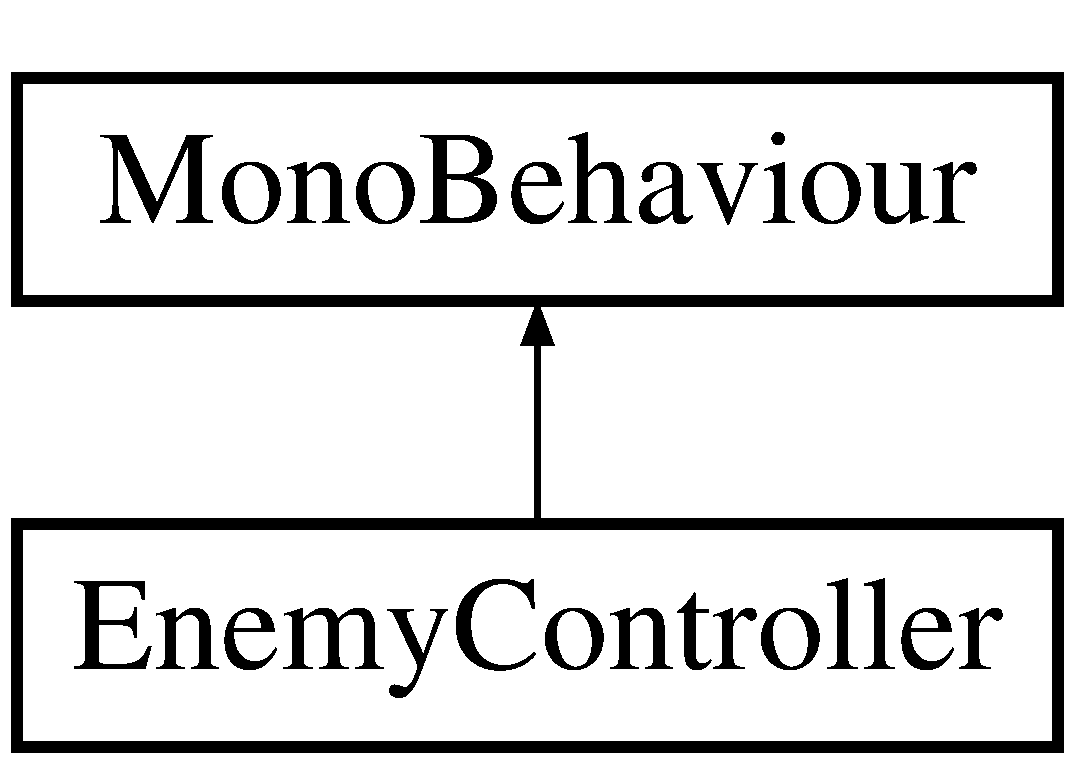
\includegraphics[height=2.000000cm]{class_enemy_controller}
\end{center}
\end{figure}
\subsection*{Classes}
\begin{DoxyCompactItemize}
\item 
class \hyperlink{class_enemy_controller_1_1_agent}{Agent}
\end{DoxyCompactItemize}
\subsection*{Public Member Functions}
\begin{DoxyCompactItemize}
\item 
\hypertarget{class_enemy_controller_a068a88160e180f49bdc2da319db95b41}{}void {\bfseries report\+Enemy} (Game\+Object go)\label{class_enemy_controller_a068a88160e180f49bdc2da319db95b41}

\item 
\hypertarget{class_enemy_controller_a730852dd7b6474fe350dc9cd791a2f91}{}void {\bfseries update\+Agent} (float agg, float def)\label{class_enemy_controller_a730852dd7b6474fe350dc9cd791a2f91}

\item 
\hypertarget{class_enemy_controller_a9c542aad48c09e7fd588763014010007}{}void {\bfseries remove\+Unit} (Game\+Object unit)\label{class_enemy_controller_a9c542aad48c09e7fd588763014010007}

\end{DoxyCompactItemize}
\subsection*{Public Attributes}
\begin{DoxyCompactItemize}
\item 
\hypertarget{class_enemy_controller_a97ab04e3ac6701654fc012b8c9b0ba31}{}\hyperlink{class_enemy_controller_1_1_agent}{Agent} {\bfseries agent}\label{class_enemy_controller_a97ab04e3ac6701654fc012b8c9b0ba31}

\end{DoxyCompactItemize}


The documentation for this class was generated from the following file\+:\begin{DoxyCompactItemize}
\item 
Assets/\+Scripts/Enemy\+Controller.\+cs\end{DoxyCompactItemize}

\hypertarget{class_game_controller}{}\section{Game\+Controller Class Reference}
\label{class_game_controller}\index{Game\+Controller@{Game\+Controller}}
Inheritance diagram for Game\+Controller\+:\begin{figure}[H]
\begin{center}
\leavevmode
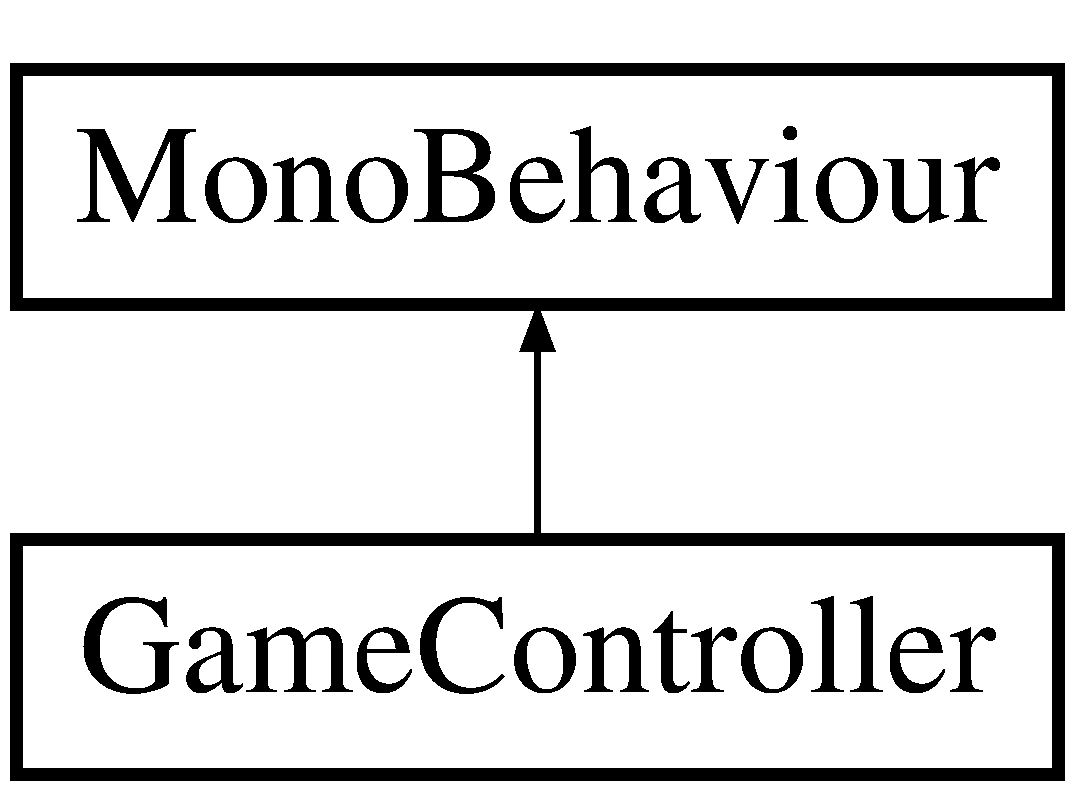
\includegraphics[height=2.000000cm]{class_game_controller}
\end{center}
\end{figure}
\subsection*{Classes}
\begin{DoxyCompactItemize}
\item 
class \hyperlink{class_game_controller_1_1_player}{Player}
\end{DoxyCompactItemize}
\subsection*{Public Types}
\begin{DoxyCompactItemize}
\item 
\hypertarget{class_game_controller_ab937754651a2f755bd6ae099c7a43a10}{}enum {\bfseries Unit\+Type} \{ \\*
{\bfseries Mothership} = 0, 
{\bfseries Destroyer}, 
{\bfseries Cruiser}, 
{\bfseries Fighter}, 
\\*
{\bfseries Transporter}, 
{\bfseries Shuttle}, 
{\bfseries Unknown}
 \}\label{class_game_controller_ab937754651a2f755bd6ae099c7a43a10}

\item 
\hypertarget{class_game_controller_a532443f5d4c5992fecce2943dc627a89}{}enum {\bfseries Game\+State} \{ \\*
{\bfseries Not\+Started}, 
{\bfseries Playing}, 
{\bfseries Paused}, 
{\bfseries Player\+Won}, 
\\*
{\bfseries Enemy\+Won}, 
{\bfseries Draw}
 \}\label{class_game_controller_a532443f5d4c5992fecce2943dc627a89}

\item 
\hypertarget{class_game_controller_a2c93703a2af5124f070ee30361edd812}{}enum {\bfseries Who} \{ {\bfseries Player}, 
{\bfseries Enemy}
 \}\label{class_game_controller_a2c93703a2af5124f070ee30361edd812}

\item 
\hypertarget{class_game_controller_a3545f5a2e68f44c964b88e3cbb0fa6a9}{}enum {\bfseries Selected} \{ {\bfseries None}, 
{\bfseries Single}, 
{\bfseries Group}
 \}\label{class_game_controller_a3545f5a2e68f44c964b88e3cbb0fa6a9}

\end{DoxyCompactItemize}
\subsection*{Public Member Functions}
\begin{DoxyCompactItemize}
\item 
\hypertarget{class_game_controller_a7533fd7506ef2ef51f35050cbf109c20}{}void {\bfseries navigate\+To} (Game\+Object unit, Vector3 pos)\label{class_game_controller_a7533fd7506ef2ef51f35050cbf109c20}

\item 
\hypertarget{class_game_controller_a19eacaf7b7a58d12ef03508959eb44d5}{}void {\bfseries navigate\+To} (List$<$ Game\+Object $>$ units, Vector3 pos)\label{class_game_controller_a19eacaf7b7a58d12ef03508959eb44d5}

\item 
\hypertarget{class_game_controller_a28daa03c0d2d957778106d03c9519ccc}{}void {\bfseries attack\+Unit} (Game\+Object unit, Game\+Object enemy)\label{class_game_controller_a28daa03c0d2d957778106d03c9519ccc}

\item 
\hypertarget{class_game_controller_a30a6c11927455a2680e61439844ea9d6}{}void {\bfseries attack\+Unit} (List$<$ Game\+Object $>$ units, Game\+Object enemy)\label{class_game_controller_a30a6c11927455a2680e61439844ea9d6}

\item 
\hypertarget{class_game_controller_ac24bfe50e36d1f80f2bb713b35950da4}{}void {\bfseries move\+Camera} (Vector3 pos)\label{class_game_controller_ac24bfe50e36d1f80f2bb713b35950da4}

\item 
\hypertarget{class_game_controller_a0a08dc740a2404be333418899e702fb9}{}void {\bfseries give\+Points\+For\+Killing} (Game\+Object unit)\label{class_game_controller_a0a08dc740a2404be333418899e702fb9}

\item 
\hypertarget{class_game_controller_af3c1116017242ec65bb53045f32447f6}{}void {\bfseries handle\+Building} (\hyperlink{class_asteroid_controller}{Asteroid\+Controller} ac)\label{class_game_controller_af3c1116017242ec65bb53045f32447f6}

\item 
\hypertarget{class_game_controller_a81d580922a9967dadf5c777c2a9a004f}{}void {\bfseries handle\+Asteroid} (Game\+Object asteroid)\label{class_game_controller_a81d580922a9967dadf5c777c2a9a004f}

\item 
\hypertarget{class_game_controller_ae1cb09c065288c83179440a8c7132672}{}void {\bfseries handle\+Game} ()\label{class_game_controller_ae1cb09c065288c83179440a8c7132672}

\item 
\hypertarget{class_game_controller_a6beec252fc2cf4bbeb8cec79d5174374}{}void {\bfseries delete\+Unit} (Game\+Object unit)\label{class_game_controller_a6beec252fc2cf4bbeb8cec79d5174374}

\item 
\hypertarget{class_game_controller_af2a993666311cdea53c950859c713e35}{}bool {\bfseries build\+Unit} (Who who, Unit\+Type type\+Of\+Unit, Vector3 position)\label{class_game_controller_af2a993666311cdea53c950859c713e35}

\item 
\hypertarget{class_game_controller_a6969a4feb3cbc18212954e0bb7e2e3cd}{}void {\bfseries deselect\+All\+Units} ()\label{class_game_controller_a6969a4feb3cbc18212954e0bb7e2e3cd}

\item 
\hypertarget{class_game_controller_ae3722a2af86bf28e6152de6f9ed802c8}{}void {\bfseries deselect\+Unit} (Game\+Object unit)\label{class_game_controller_ae3722a2af86bf28e6152de6f9ed802c8}

\item 
\hypertarget{class_game_controller_a9a5e2e7359a2d77423644c92678154d2}{}void {\bfseries select\+Unit} (Game\+Object unit)\label{class_game_controller_a9a5e2e7359a2d77423644c92678154d2}

\item 
\hypertarget{class_game_controller_a4fb46a1b2d3b5132ef792f81db466586}{}void {\bfseries add\+To\+Group} (Game\+Object unit)\label{class_game_controller_a4fb46a1b2d3b5132ef792f81db466586}

\item 
\hypertarget{class_game_controller_ab1219cdc405982b5e9947e004fef207b}{}Game\+Object {\bfseries get\+Selected\+Unit} ()\label{class_game_controller_ab1219cdc405982b5e9947e004fef207b}

\item 
\hypertarget{class_game_controller_ab9fb961e72e2bd99bb3da82988143a23}{}List$<$ Game\+Object $>$ {\bfseries get\+Selected\+Group} ()\label{class_game_controller_ab9fb961e72e2bd99bb3da82988143a23}

\end{DoxyCompactItemize}
\subsection*{Static Public Member Functions}
\begin{DoxyCompactItemize}
\item 
\hypertarget{class_game_controller_ae3f5a83f04b65f5a56538bcf4e04f0b6}{}static Unit\+Type {\bfseries get\+Unit\+Type} (Game\+Object ob)\label{class_game_controller_ae3f5a83f04b65f5a56538bcf4e04f0b6}

\end{DoxyCompactItemize}
\subsection*{Public Attributes}
\begin{DoxyCompactItemize}
\item 
\hypertarget{class_game_controller_a674085d39c0f50688fe9af5f9596d806}{}\hyperlink{class_game_controller_1_1_player}{Player}\mbox{[}$\,$\mbox{]} {\bfseries players}\label{class_game_controller_a674085d39c0f50688fe9af5f9596d806}

\item 
\hypertarget{class_game_controller_aa81cbf39eea608ee93dc76c572b42195}{}Game\+Object\mbox{[}$\,$\mbox{]} {\bfseries asteroids}\label{class_game_controller_aa81cbf39eea608ee93dc76c572b42195}

\item 
\hypertarget{class_game_controller_a129b256ff0d239cac52dbc5882f147b1}{}const int {\bfseries type\+Of\+Units} = 7\label{class_game_controller_a129b256ff0d239cac52dbc5882f147b1}

\item 
\hypertarget{class_game_controller_a7d09c64261bcee941e31fe9b1db7272c}{}float\mbox{[}$\,$\mbox{]} {\bfseries unit\+Costs} = new float\mbox{[}type\+Of\+Units\mbox{]}\label{class_game_controller_a7d09c64261bcee941e31fe9b1db7272c}

\item 
\hypertarget{class_game_controller_aeb780e3e7da55b2127fee53ee5ee3d81}{}Game\+Object\mbox{[}$\,$\mbox{]} {\bfseries unit\+Prefabs} = new Game\+Object\mbox{[}type\+Of\+Units\mbox{]}\label{class_game_controller_aeb780e3e7da55b2127fee53ee5ee3d81}

\item 
\hypertarget{class_game_controller_a994169e702283f71d719b2e6889153f1}{}Game\+Object\mbox{[}$\,$\mbox{]} {\bfseries enemy\+Prefabs} = new Game\+Object\mbox{[}type\+Of\+Units\mbox{]}\label{class_game_controller_a994169e702283f71d719b2e6889153f1}

\end{DoxyCompactItemize}


The documentation for this class was generated from the following file\+:\begin{DoxyCompactItemize}
\item 
C\+:/\+Users/\+Franek/\+Documents/\+Cast into the Voidstar/\+Assets/\+Scripts/Game\+Controller.\+cs\end{DoxyCompactItemize}

\hypertarget{class_game_controller_1_1_player}{}\section{Game\+Controller.\+Player Class Reference}
\label{class_game_controller_1_1_player}\index{Game\+Controller.\+Player@{Game\+Controller.\+Player}}
\subsection*{Public Member Functions}
\begin{DoxyCompactItemize}
\item 
\hypertarget{class_game_controller_1_1_player_ab1bb535287a6effa0bf6062541491782}{}void {\bfseries add\+Unit} (Game\+Object ob)\label{class_game_controller_1_1_player_ab1bb535287a6effa0bf6062541491782}

\item 
\hypertarget{class_game_controller_1_1_player_a2583776006e097e47a62704dc2cd1520}{}void {\bfseries remove\+Unit} (Game\+Object ob)\label{class_game_controller_1_1_player_a2583776006e097e47a62704dc2cd1520}

\item 
\hypertarget{class_game_controller_1_1_player_a9736a162383edd80db08b704db75c6ba}{}int {\bfseries get\+Unit\+Count} (Unit\+Type type)\label{class_game_controller_1_1_player_a9736a162383edd80db08b704db75c6ba}

\item 
\hypertarget{class_game_controller_1_1_player_a52084561e9cb975d963c444af033c479}{}void {\bfseries set\+Points} (float p)\label{class_game_controller_1_1_player_a52084561e9cb975d963c444af033c479}

\item 
\hypertarget{class_game_controller_1_1_player_ac758424ac07c5cc7205bad34ed071e8e}{}float {\bfseries get\+Points} ()\label{class_game_controller_1_1_player_ac758424ac07c5cc7205bad34ed071e8e}

\item 
\hypertarget{class_game_controller_1_1_player_a56a46f8663199c0b25608f10d168512a}{}void {\bfseries set\+Credits} (float c)\label{class_game_controller_1_1_player_a56a46f8663199c0b25608f10d168512a}

\item 
\hypertarget{class_game_controller_1_1_player_a7699a0b5104492b29d3eabab0395c850}{}float {\bfseries get\+Credits} ()\label{class_game_controller_1_1_player_a7699a0b5104492b29d3eabab0395c850}

\end{DoxyCompactItemize}
\subsection*{Static Public Member Functions}
\begin{DoxyCompactItemize}
\item 
\hypertarget{class_game_controller_1_1_player_a0e2648f9c886f3ca4b7484f96694187d}{}static Unit\+Type {\bfseries get\+Unit\+Type} (Game\+Object ob)\label{class_game_controller_1_1_player_a0e2648f9c886f3ca4b7484f96694187d}

\end{DoxyCompactItemize}


The documentation for this class was generated from the following file\+:\begin{DoxyCompactItemize}
\item 
Assets/\+Scripts/Game\+Controller.\+cs\end{DoxyCompactItemize}

\hypertarget{class_shot}{}\section{Shot Class Reference}
\label{class_shot}\index{Shot@{Shot}}
Inheritance diagram for Shot\+:\begin{figure}[H]
\begin{center}
\leavevmode
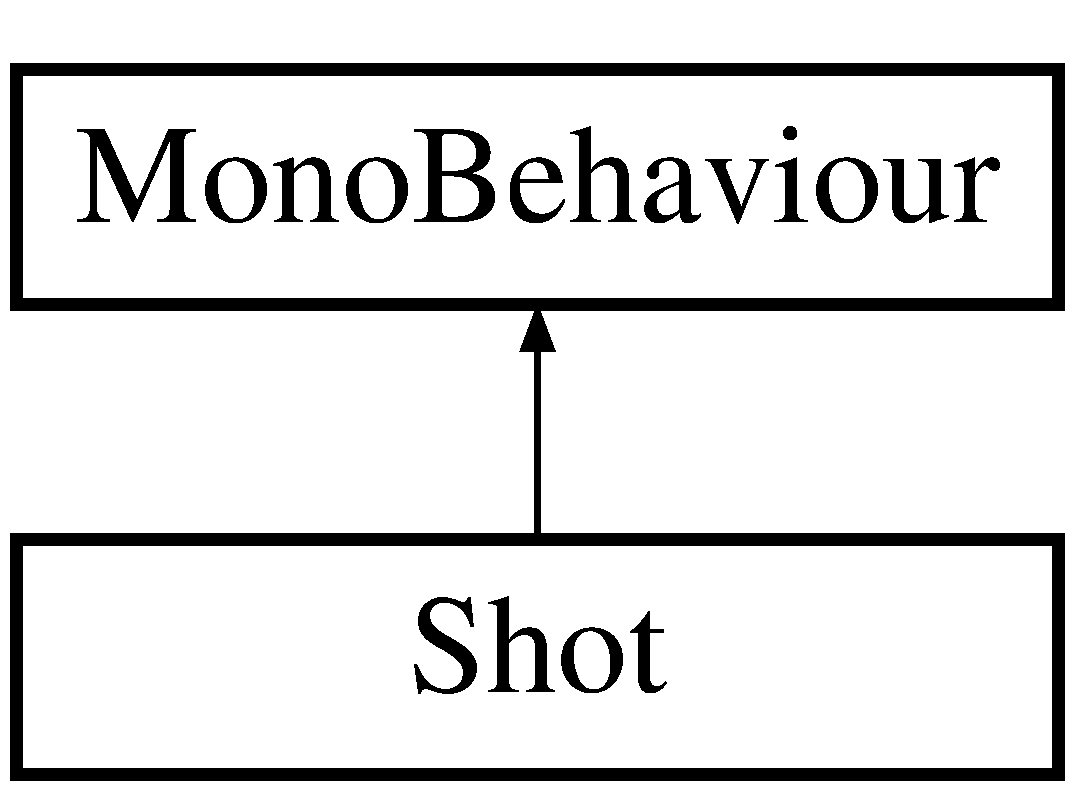
\includegraphics[height=2.000000cm]{class_shot}
\end{center}
\end{figure}
\subsection*{Public Member Functions}
\begin{DoxyCompactItemize}
\item 
\hypertarget{class_shot_a1c90a6a43a28389266ab330a1d5cce39}{}void {\bfseries fire} (float dmg)\label{class_shot_a1c90a6a43a28389266ab330a1d5cce39}

\item 
\hypertarget{class_shot_a19a65826fd2946bf518662f13ace77d9}{}void {\bfseries set\+Owner} (Game\+Object go)\label{class_shot_a19a65826fd2946bf518662f13ace77d9}

\end{DoxyCompactItemize}
\subsection*{Public Attributes}
\begin{DoxyCompactItemize}
\item 
\hypertarget{class_shot_ab122de347dcdf571ce02344e0900bc6b}{}float {\bfseries fire\+Force} = 1000.\+0f\label{class_shot_ab122de347dcdf571ce02344e0900bc6b}

\item 
\hypertarget{class_shot_a45f3d0367ce3e6dc6025e2a771256c35}{}float {\bfseries damage} = 50.\+0f\label{class_shot_a45f3d0367ce3e6dc6025e2a771256c35}

\end{DoxyCompactItemize}


The documentation for this class was generated from the following file\+:\begin{DoxyCompactItemize}
\item 
C\+:/\+Users/\+Franek/\+Documents/\+Cast into the Voidstar/\+Assets/\+Scripts/Shot.\+cs\end{DoxyCompactItemize}

\hypertarget{class_unit_controller}{}\section{Unit\+Controller Class Reference}
\label{class_unit_controller}\index{Unit\+Controller@{Unit\+Controller}}
Inheritance diagram for Unit\+Controller\+:\begin{figure}[H]
\begin{center}
\leavevmode
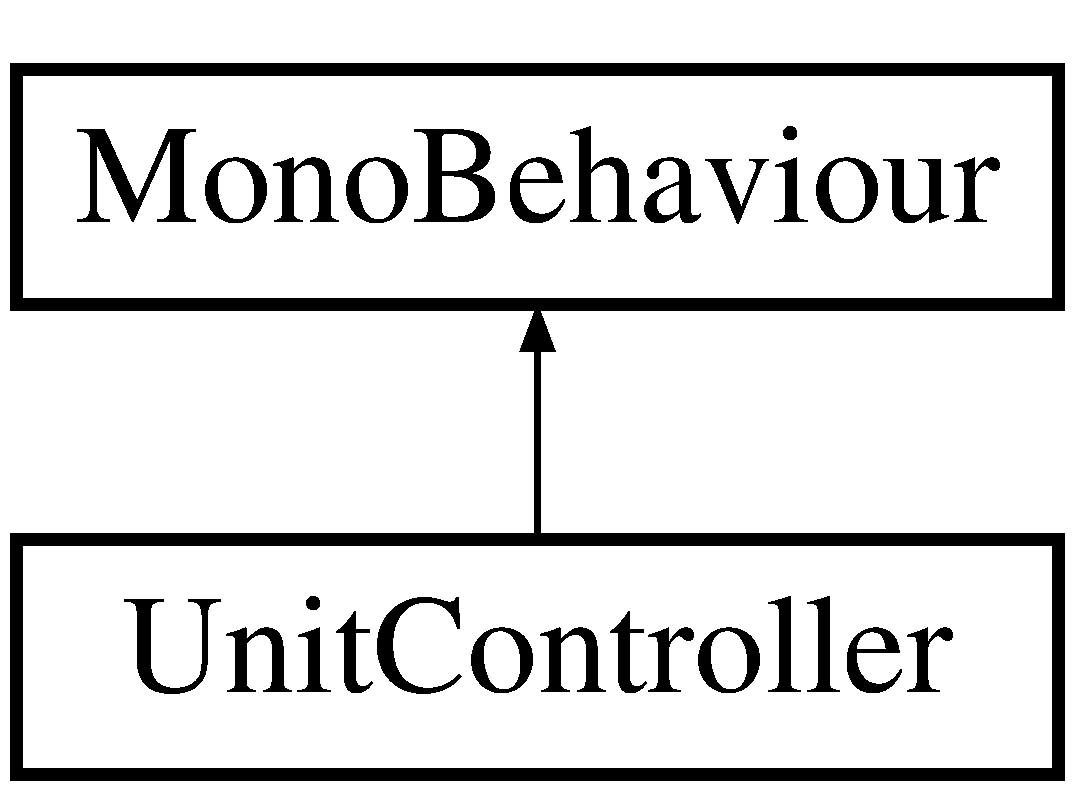
\includegraphics[height=2.000000cm]{class_unit_controller}
\end{center}
\end{figure}
\subsection*{Public Member Functions}
\begin{DoxyCompactItemize}
\item 
\hypertarget{class_unit_controller_a94132ec1f2ffd7bf1e224ea24fecf9e6}{}void {\bfseries set\+Target} (Game\+Object go)\label{class_unit_controller_a94132ec1f2ffd7bf1e224ea24fecf9e6}

\item 
\hypertarget{class_unit_controller_ab6381f8b8da8f0509f23bda9871a5e90}{}void {\bfseries move\+To} (Vector3 pos)\label{class_unit_controller_ab6381f8b8da8f0509f23bda9871a5e90}

\item 
\hypertarget{class_unit_controller_a4b7718e2d007cc652601dec1654136c2}{}void {\bfseries fire} ()\label{class_unit_controller_a4b7718e2d007cc652601dec1654136c2}

\item 
\hypertarget{class_unit_controller_a1a29d3f3d0bd4166f0094103f6c5a7e7}{}void {\bfseries attack} (Game\+Object go)\label{class_unit_controller_a1a29d3f3d0bd4166f0094103f6c5a7e7}

\item 
\hypertarget{class_unit_controller_a650b7ed580602a0e2d18b3e64cc7daa1}{}float {\bfseries get\+Attack\+Force} ()\label{class_unit_controller_a650b7ed580602a0e2d18b3e64cc7daa1}

\item 
\hypertarget{class_unit_controller_ae81b8f04d34b104eb9d73f353cf275de}{}float {\bfseries get\+Hit\+Points} ()\label{class_unit_controller_ae81b8f04d34b104eb9d73f353cf275de}

\item 
\hypertarget{class_unit_controller_a9b8260bff2cb66c92aacb71b5e96529f}{}void {\bfseries set\+Hit\+Points} (float f)\label{class_unit_controller_a9b8260bff2cb66c92aacb71b5e96529f}

\item 
\hypertarget{class_unit_controller_abd5e7ad90a255e0f0103ddc312df4bb9}{}void {\bfseries die} ()\label{class_unit_controller_abd5e7ad90a255e0f0103ddc312df4bb9}

\end{DoxyCompactItemize}
\subsection*{Public Attributes}
\begin{DoxyCompactItemize}
\item 
\hypertarget{class_unit_controller_a8fb130f3cd6edb7e866cfa1053c3d524}{}Game\+Object {\bfseries shot}\label{class_unit_controller_a8fb130f3cd6edb7e866cfa1053c3d524}

\item 
\hypertarget{class_unit_controller_a24e925167637d0e1d2220d62bb9cb964}{}Transform {\bfseries shot\+Spawn}\label{class_unit_controller_a24e925167637d0e1d2220d62bb9cb964}

\end{DoxyCompactItemize}


The documentation for this class was generated from the following file\+:\begin{DoxyCompactItemize}
\item 
C\+:/\+Users/\+Franek/\+Documents/\+Cast into the Voidstar/\+Assets/\+Scripts/Unit\+Controller.\+cs\end{DoxyCompactItemize}

%--- End generated contents ---

% Index
\backmatter
\newpage
\phantomsection
\clearemptydoublepage
\addcontentsline{toc}{chapter}{Index}
\printindex

\end{document}
